\documentclass[a4paper,11pt]{scrbook}
\usepackage{fancyhdr}
\usepackage[a4paper,top=2cm,bottom=2cm]{geometry}
\usepackage{graphicx}
\setlength{\voffset}{0.5in}
\setlength{\oddsidemargin}{28pt}
\setlength{\evensidemargin}{0pt}
\renewcommand{\footrulewidth}{0.5pt}
\lhead[\fancyplain{}{\Large \thepage}]%
      {\fancyplain{}{\rightmark}}
\rhead[\fancyplain{}{\leftmark}]%
      {\fancyplain{}{\Large \thepage}}
\pagestyle{fancy}
\lfoot[\emph{Pemberkatan rumah}]{}
\rfoot[]{\emph{Kel. Th Totok Suyanto}}
\cfoot{}
\topmargin=-0.5in
\textheight=9in
%\sloppy


\makeatletter
\newcommand{\judul}[1]{%
  {\parindent \z@ \centering 
    \interlinepenalty\@M \Large \bfseries #1\par\nobreak \vskip 20\p@ }}
\newcommand{\subjudul}[1]{%
  {\parindent \z@ 
    \interlinepenalty\@M \bfseries #1\par\nobreak \vskip 10\p@ }}
\newcommand{\lagu}[1]{%
  {\parindent \z@ 
    \interlinepenalty\@M \bfseries \textsl{#1}\par\nobreak \vskip 20\p@ }}
\newcommand{\keterangan}[1]{%
  {\parindent \z@  \slshape \large
    \interlinepenalty\@M \textsl{#1}\par\nobreak  \vskip 5\p@}}

\renewenvironment{description}
               {\list{}{\labelwidth\z@ \itemindent-\leftmargin
                        \let\makelabel\descriptionlabel}}
               {\endlist}
\renewcommand*\descriptionlabel[1]{\hspace\labelsep 
                                \normalfont\bfseries #1 }

\hyphenation{a-kan}
\hyphenation{ba-gi-mu}
\hyphenation{ber-a-da}
\hyphenation{ber-du-a}
\hyphenation{be-ri-kan}
\hyphenation{ber-ka-ta}
\hyphenation{ber-nya-nyi}
\hyphenation{ber-sa-ma}

\hyphenation{dah-syat}
\hyphenation{DA-RAH-KU}
\hyphenation{da-tang}
\hyphenation{di-ka-ta-kan}
\hyphenation{di-pim-pin}
\hyphenation{di-se-rah-kan}
\hyphenation{di-tum-pah-kan}

\hyphenation{Eng-kau}
\hyphenation{ha-dap-an}
\hyphenation{han-tar-kan-lah}
\hyphenation{ha-rap-an}

\hyphenation{ja-lan}
\hyphenation{ja-ngan-lah}

\hyphenation{ka-nak}
\hyphenation{ka-re-na}
\hyphenation{kau-lim-pah-kan}
\hyphenation{Kau-cip-ta-kan}
\hyphenation{ke-bang-kit-an-Nya}
\hyphenation{ke-da-tang-an}
\hyphenation{ke-da-tang-an-Nya}
\hyphenation{ke-dua}
\hyphenation{ke-na-ik-kan-nya}
\hyphenation{ke-pa-daMu}
\hyphenation{ke-ra-him-an}
\hyphenation{ke-se-jah-te-ra-an-mu}
\hyphenation{ko-men-tar}

\hyphenation{la-ma-nya}
\hyphenation{lim-pah-kan}

\hyphenation{ma-nu-sia}
\hyphenation{me-nga-da-kan}
\hyphenation{me-ngan-dung-lah}
\hyphenation{me-ngu-kuh-kan}
\hyphenation{me-la-lui}
\hyphenation{me-lim-pah-kan}
\hyphenation{me-lu-hur-kan}
\hyphenation{me-me-cah-me-cah-kan}
\hyphenation{mem-per-sem-bah-kan}
\hyphenation{me-nan-da-ta-ngan-i}
\hyphenation{men-cin-tai}
\hyphenation{meng-a-lir-kan}
\hyphenation{me-nga-sihi}
\hyphenation{me-nge-lu-ar-kan}
\hyphenation{meng-u-cap-kan}
\hyphenation{meng-ung-kap-kan}
\hyphenation{me-num-buh-kan}
\hyphenation{me-nya-ta-kan}
\hyphenation{me-nye-la-mat-kan}
\hyphenation{me-nye-rah-kan}
\hyphenation{me-nye-rah-kanNya}
\hyphenation{me-ra-ya-kan}

\hyphenation{o-rang}
\hyphenation{o-rang-o-rang}

\hyphenation{pa-sang-kan-lah}
\hyphenation{pa-tut}
\hyphenation{pe-ne-ri-ma-an}
\hyphenation{pe-ngam-pun-an}
\hyphenation{Pe-ngan-ta-ra}
\hyphenation{peng-hi-bur-an}
\hyphenation{per-bu-at-an-nya}
\hyphenation{per-ka-ta-an}
\hyphenation{per-ka-win-an}
\hyphenation{per-ni-kah-an}
\hyphenation{per-se-ku-tu-an}
\hyphenation{per-sem-bah-an}
\hyphenation{rom-bong-an}

\hyphenation{se-la-ma}
\hyphenation{se-ka-li-an}
\hyphenation{se-pan-jang}
\hyphenation{se-ra-ya}
\hyphenation{Su-dar-yan-to}

\hyphenation{te-ta-pi}
\hyphenation{ta-ngan-Mu}
\hyphenation{Tu-han}
\hyphenation{tu-lang}
\hyphenation{tu-lang-tu-lang}

\hyphenation{u-mat-Mu}
\hyphenation{wa-kil}

\hyphenation{ba-gi-mu}
\hyphenation{di-se-rah-kan}
\hyphenation{me-la-lui}
\hyphenation{ka-nak}
\hyphenation{ka-re-na}
\hyphenation{ber-ka-ta}
\hyphenation{te-ta-pi}
\hyphenation{per-ka-win-an}
\hyphenation{pa-tut}
\hyphenation{me-lu-hur-kan}
\hyphenation{ber-nya-nyi}
\hyphenation{di-tum-pah-kan}
\hyphenation{pe-ngam-pun-an}
\hyphenation{ber-a-da}
\hyphenation{kau-lim-pah-kan}
\hyphenation{ke-bang-kit-an-Nya}
\hyphenation{per-ka-ta-an}
\hyphenation{pa-sang-kan-lah}
\hyphenation{DA-RAH-KU}
\hyphenation{ke-na-ik-kan-nya}
\hyphenation{per-sem-bah-an}
\hyphenation{per-se-ku-tu-an}



\makeatother

\newcommand{\BU}[1]{\begin{itemize} \item[U:] #1 \end{itemize}}
\newcommand{\BI}[1]{\begin{itemize} \item[I:] #1 \end{itemize}}
\newcommand{\BP}[1]{\begin{itemize} \item[P:] #1 \end{itemize}}

\newcommand{\keluarga}{Theodorus Totok Suyanto }
\newcommand{\romo}{Ign Yulianto, OMI }

%lagu-lagu
%\newcommand{\lagupembukaan}{Hatiku Gembira - MB 172}
%\newcommand{\lagukyrie}{MB 186 }
%\newcommand{\lagugloria}{~}
%\newcommand{\laguantarbacaan}{Bahagia Manusia - MB 214 }
\newcommand{\lagupembukaan}{~}
\newcommand{\lagukyrie}{~ }
\newcommand{\lagugloria}{~}
\newcommand{\laguantarbacaan}{~ }
\newcommand{\lagupersembahan}{Betapa Hatiku }
\newcommand{\lagurecikan}{Tuhan Rajaku - MB 503}
\newcommand{\lagusanctus}{~ }
\newcommand{\lagubapakami}{~ }
\newcommand{\laguagnusdei}{MB 278 }
\newcommand{\lagukomuni}{Kumau Cinta Yesus (\textsl{Asri Savsavubun})\\
                         Intrumen dengan biola (\textsl{Morits})}
\newcommand{\lagupenutup}{O Sanctisima }


\usepackage[bahasa]{babel}
\selectlanguage{bahasa}

\title{EKARISTI \\PEMBERKATAN RUMAH}
\author{
%
\includegraphics[scale=2]{ill044}\\
Keluarga \keluarga \\ \\
%leh Romo \romo
} 
\date{20 Mei 2009}
\begin{document}
\sffamily
\maketitle
\LARGE  
\thispagestyle{empty}
%\newpage
%~~~ 
\newpage
\judul{RITUS PEMBUKA}

\lagu{Lagu pembukaan \lagupembukaan}

\subjudul{Tanda Salib}
\BI{Dalam nama Bapa dan Putera dan Roh Kudus}
\BU{Amin}

\subjudul{Salam Pembukaan}
\BI{Rahmat Tuhan kita Yesus Kristus, cinta kasih Allah, dan persekutuan Roh Kudus beserta kita}
\BU{Sekarang dan selama-lamanya}

\subjudul{Pengantar}
\BI{Bapak, Ibu, dan Saudara-saudara, berkat sakramen pembaptisan Tuhan telah berkenan datang dan hadir di dalam diri kita. Kedatangan dan kehadiran Tuhan itu selalu diperbaharui secara khusus setiap kali kita menerima sakramen. 

Di dalam sakramen perkawinan Tuhan malahan datang di tengah-tengah keluarga kita. Tetapi pada kesempatan ini kita diundang keluarga Bapak \keluarga untuk mohon berkat bagi rumah ini, agar pergaulan dan pekerjaan kita di sini diberkati dan direstui oleh Tuhan dan berkenan di hati-Nya.}

\subjudul{Tobat}
\BI{Marilah kita hening sejenak untuk mempersiapkan diri dalam perayaan syukur ini sambil menyadari bahwa kita sering melupakan kebaikan Tuhan dan enggan mewartakan dan mewujudkan kebaikan tersebut melalui pikiran, perkataan, dan perbuatan kita.}

\BI{Saya mengaku}

\BU{Kepada Allah yang Maha Kuasa dan kepada saudara sekalian bahwa saya telah berdosa dengan pikiran dan perkataan, dengan perbuatan dan kelalaian. Saya berdosa, saya berdosa, saya sungguh berdosa. Oleh sebab itu saya mohon kepada Santa Perawan Maria, kepada Para Malaikat dan orang kudus dan kepada saudara sekalian, supaya mendoakan saya kepada Allah Tuhan kita.}

\BI{Semoga Allah Yang Maha Kuasa mengasihi kita, mengampuni dosa kita dan menghantar kita ke hidup yang kekal.}

\BU{Amin}

\lagu{Tuhan Kasihanilah Kami}

\subjudul{Doa Pembukaan}

\BI{Marilah kita berdoa,
Allah yang mahakuasa, Bapa maha pengasih, sudilah memberkati dan melindungi keluarga ini. Bimbinglah kami selalu supaya hidup rukun, sayang-menyayangi, hormat-menghormati, tolong-menolong, bijaksana dan sederhana. Dengan demikian kami akan semakin berkenan di hati-Mu serta memberi kesaksian atas karya penyelamatan-Mu. Demi Kristus, Tuhan dan pengantara kami.}

\BU{Amin}

\judul{LITURGI SABDA}

\subjudul{Bacaan pertama: Kej 18:1-10a}

\BP{\emph{Pembacaan dari Kitab Kejadian.}

Kemudian TUHAN menampakkan diri kepada Abraham dekat pohon tarbantin di Mamre, sedang ia duduk di pintu kemahnya waktu hari panas terik.
Ketika ia mengangkat mukanya, ia melihat tiga orang berdiri di depannya. Sesudah dilihatnya mereka, ia berlari dari pintu kemahnya menyongsong mereka, lalu sujudlah ia sampai ke tanah,
serta berkata: "Tuanku, jika aku telah mendapat kasih tuanku, janganlah kiranya lampaui hambamu ini.
Biarlah diambil air sedikit, basuhlah kakimu dan duduklah beristirahat di bawah pohon ini;
biarlah kuambil sepotong roti, supaya tuan-tuan segar kembali; kemudian bolehlah tuan-tuan meneruskan perjalanannya; sebab tuan-tuan telah datang ke tempat hambamu ini." Jawab mereka: "Perbuatlah seperti yang kaukatakan itu."

Lalu Abraham segera pergi ke kemah mendapatkan Sara serta berkata: "Segeralah! Ambil tiga sukat tepung yang terbaik! Remaslah itu dan buatlah roti bundar!"

Lalu berlarilah Abraham kepada lembu sapinya, ia mengambil seekor anak lembu yang empuk dan baik dagingnya dan memberikannya kepada seorang bujangnya, lalu orang ini segera mengolahnya.
Kemudian diambilnya dadih dan susu serta anak lembu yang telah diolah itu, lalu dihidangkannya di depan orang-orang itu; dan ia berdiri di dekat mereka di bawah pohon itu, sedang mereka makan.

Lalu kata mereka kepadanya: "Di manakah Sara, isterimu?" Jawabnya: "Di sana, di dalam kemah."
Dan firman-Nya: "Sesungguhnya Aku akan kembali tahun depan mendapatkan engkau, pada waktu itulah Sara, isterimu, akan mempunyai seorang anak laki-laki." 

\emph{Demikianlah sabda Tuhan}
}

\BU{Syukur kepada Allah.}

\lagu{Lagu Pengantar Bacaan: \laguantarbacaan}

\lagu{Bait Pengantar Injil}

\subjudul{Bacaan Injil: Lukas 19: 1 - 9}

\BI{Tuhan sertamu}

\BU{Dan sertamu juga}

\BI{Inilah Injil Yesus Kristus menurut Santo Lukas}

\BU{Dimuliakanlah Tuhan}

\BI{
Yesus masuk ke kota Yerikho dan berjalan terus melintasi kota itu.
Di situ ada seorang bernama Zakheus, kepala pemungut cukai, dan ia seorang yang kaya.
Ia berusaha untuk melihat orang apakah Yesus itu, tetapi ia tidak berhasil karena orang banyak, sebab badannya pendek.
Maka berlarilah ia mendahului orang banyak, lalu memanjat pohon ara untuk melihat Yesus, yang akan lewat di situ.
Ketika Yesus sampai ke tempat itu, Ia melihat ke atas dan berkata: "Zakheus, segeralah turun, sebab hari ini Aku harus menumpang di rumahmu."
Lalu Zakheus segera turun dan menerima Yesus dengan sukacita.
Tetapi semua orang yang melihat hal itu bersungut-sungut, katanya: "Ia menumpang di rumah orang berdosa."
Tetapi Zakheus berdiri dan berkata kepada Tuhan: "Tuhan, setengah dari milikku akan kuberikan kepada orang miskin dan sekiranya ada sesuatu yang kuperas dari seseorang akan kukembalikan empat kali lipat."
Kata Yesus kepadanya: "Hari ini telah terjadi keselamatan kepada rumah ini, karena orang inipun anak Abraham."

Berbahagialah orang yang mendengarkan sabda Tuhan, dan tekun melaksanakannya.}

\BU{Sabda-Mu adalah jalan, kebenaran dan hidup kami.}

\subjudul{Homili}

\subjudul{Pemberkatan}
\BI{Marilah berdoa:

Tuhan Yesus Kristus, Engkau telah memberkati rumah Zakheus. Engkau telah menyuruh para murid memberkati rumah-rumah yang mereka masuki. Dengan penuh harapan kami mohon kepada-Mu, sudilah kiranya menjadikan rumah ini tempat bernaung, beriman, kerukunan dan kedamaian bagi keluarga ini dan semua penghuninya. Berkatilah rumah ini, agar penghuninya mendapatkan cinta kasih dan damai, kesejahteraan dan suka cita sejati. Dan semoga berkat-Mu tinggal di rumah ini selamanya. Engkau yang hidup dan berkuasa kini dan sepanjang masa.}

\BU{Amin.}

\noindent{\emph{Seluruh rumah direciki air suci dapat diiringi lagu \lagurecikan}}


\subjudul{Aku Percaya}

\subjudul{Doa Umat}

\BI{Tuhan Yesus Kristus, Engkau pernah bersabda, "Zakheus, hari ini Aku akan datang ke rumahmu." Bersabdalah demikian juga kepada saudara kami \keluarga yang mendambakan berkat serta kehadiran-Mu di dalam rumahnya.}

\BP{Sudilah melimpahkan berkat-Mu atas keluarga ini dalam wujud: kesehatan, kegembiraan, kerukunan dan cinta kasih yang tulus ikhlas. Hiasilah rumah tangga ini dengan suasan enuh kedamaian, seperti keluara kudus di Nazaret, supaya semua yang tinggal di sini merasa damai dan tenteram. Kami mohon:}

\BU{Kabulkanlah doa kami, ya Tuhan.}

\BP{Jauhkanlah rumah ini dari salah faham, pertengkaran, perselisihan ataupun iri dan dengki sesama manusia. Dampingilah keluarga ini bila sekali waktu mengalami difitnah, dan jauhkanlah segala yang dapat menggoncangkan ketentraman serta keutuhan keluarga. Kami mohon:}

\BU{Kabulkanlah doa kami, ya Tuhan.}

\BP{Tuhan, berkatilah seluruh rumah ini, karena di dalamnya berdiam putera-puteri kesayanganMu. Jagalah agar rumah ini tetap kokoh berdiri, sehingga dapat menjadi naungan yang aman bagi seluruh penghuninya. Kami mohon:} 

\BU{Kabulkanlah doa kami, ya Tuhan.}

\BP{Hiasilah keluarga ini dengan sikap lemah lembut serta ramah tamah kepada sesama, dan hormat bakti kepada Allah, sehingga di dalam rumah ini orang dapat melihat pengalaman ajaran-Mu yang utama yakni: cinta kepada Allah dan kasih kepada sesama. Kami mohon:}

\BU{Kabulkanlah doa kami, ya Tuhan.}

\BP{Anugerahilah keluarga ini bagian dari kebijaksanaan-Mu yang suci, agar mereka dapat mendidik anak-anak seturut ajaran-Mu supaya anak-anak dalam keluarga ini pandai berbakti kepada Allah, penuh hormat kepada orangtua, dan berguna bagi negara serta sesama. Kami mohon:}

\BU{Kabulkanlah doa kami, ya Tuhan.}

\BP{Restuilah pekerjaan dan segala usaha keluarga ini, agar mendatangkan hasil yang memuaskan bagi kelestarian dan kesejahteraan keluarga ini. Kami mohon:}

\BU{Kabulkanlah doa kami, ya Tuhan.}

\BP{Dampingilah Bapak Ibu \keluarga yang mempimpin keluarga ini. Semoga mereka saling menunjukkan kesetiaan dan keterbukaan satu sama lain. Semoga cinta kasih mereka dari hari ke hari makin berkembang, dan memadu mereka sehati sejiwa dalam memimpin keluarga ini bersama-Mu. Kami mohon:}

\BU{Kabulkanlah doa kami, ya Tuhan.}

\BP{Bagi kami - umat yang berkumpul di sini, ya Tuhan. Semoga kami tak segan-segan menolong dan membantu sesama kami membagikan rahmat yang telah Kauanugerahkan kepada kami. Kami mohon:}

\BU{Kabulkanlah doa kami, ya Tuhan.}

\judul{LITURGI EKARISTI}

\subjudul{Persiapan Persembahan}

\lagu{Lagu persembahan}

\subjudul{Prefasi}

\lagu{Kudus}

\subjudul{Doa Syukur Agung}

\subjudul{Bapa Kami}

\subjudul{Salam Damai}

\lagu{Anak Domba Allah}

\subjudul{Persiapan Komuni}

\lagu{Lagu Komuni}

\judul{RITUS PENUTUP}

\subjudul{Ucapan Terima Kasih}

\subjudul{Berkat}

\BI{Saudara sekalian, marilah kita mengakhiri misa syukur pemberkatan rumah keluarga Bapak \keluarga dengan mohon berkat dari Tuhan.}
\BI{Tuhan sertamu}
\BU{Dan sertamu juga}
\BI{Semoga keluarga ini dan kita semua yang hadir di sini senantiasa dibimbing dan dilindungi dengan limpahan berkat dari Allah Yang Maha Baik. ($\dagger$) Atas Nama Bapa, Putra, dan Roh Kudus}
\BU{Amin}
\BI{Dengan demikian misa syukur pemberkatan rumah keluarga Bapak \keluarga ini telah selesai.}
\BU{Syukur kepada Allah.}
\BI{Marilah pergi, kita diutus}
\BU{Amin}

\lagu{Lagu penutup}
\newpage
\thispagestyle{empty}
\judul{Ucapan Terima Kasih}
\begin{center}
%
\includegraphics{images}

Dengan penuh rasa syukur kepada Allah, terima kasih yang tulus kami haturkan kepada:

Romo \romo \vspace{0.5cm}

Semua pihak yang telah membantu terselenggaranya \\
Perayaan Ekaristi Pemberkatan rumah ini.\vspace{0.5cm}

Segenap kerabat dan handai taulan yang berkenan menghadiri\\
Perayaan Ekaristi Pemberkatan rumah ini.\vspace{0.5cm}

\vspace{2cm}
\emph{\flushright 
Th. Totok Suyanto\\
M. I. Sri Rahayu\\
A. Nico Nugroho Pratama\\
Jl. Gori IV Karangnongko\\
RT 09 / RW 14 Maguwoharjo\\
}
%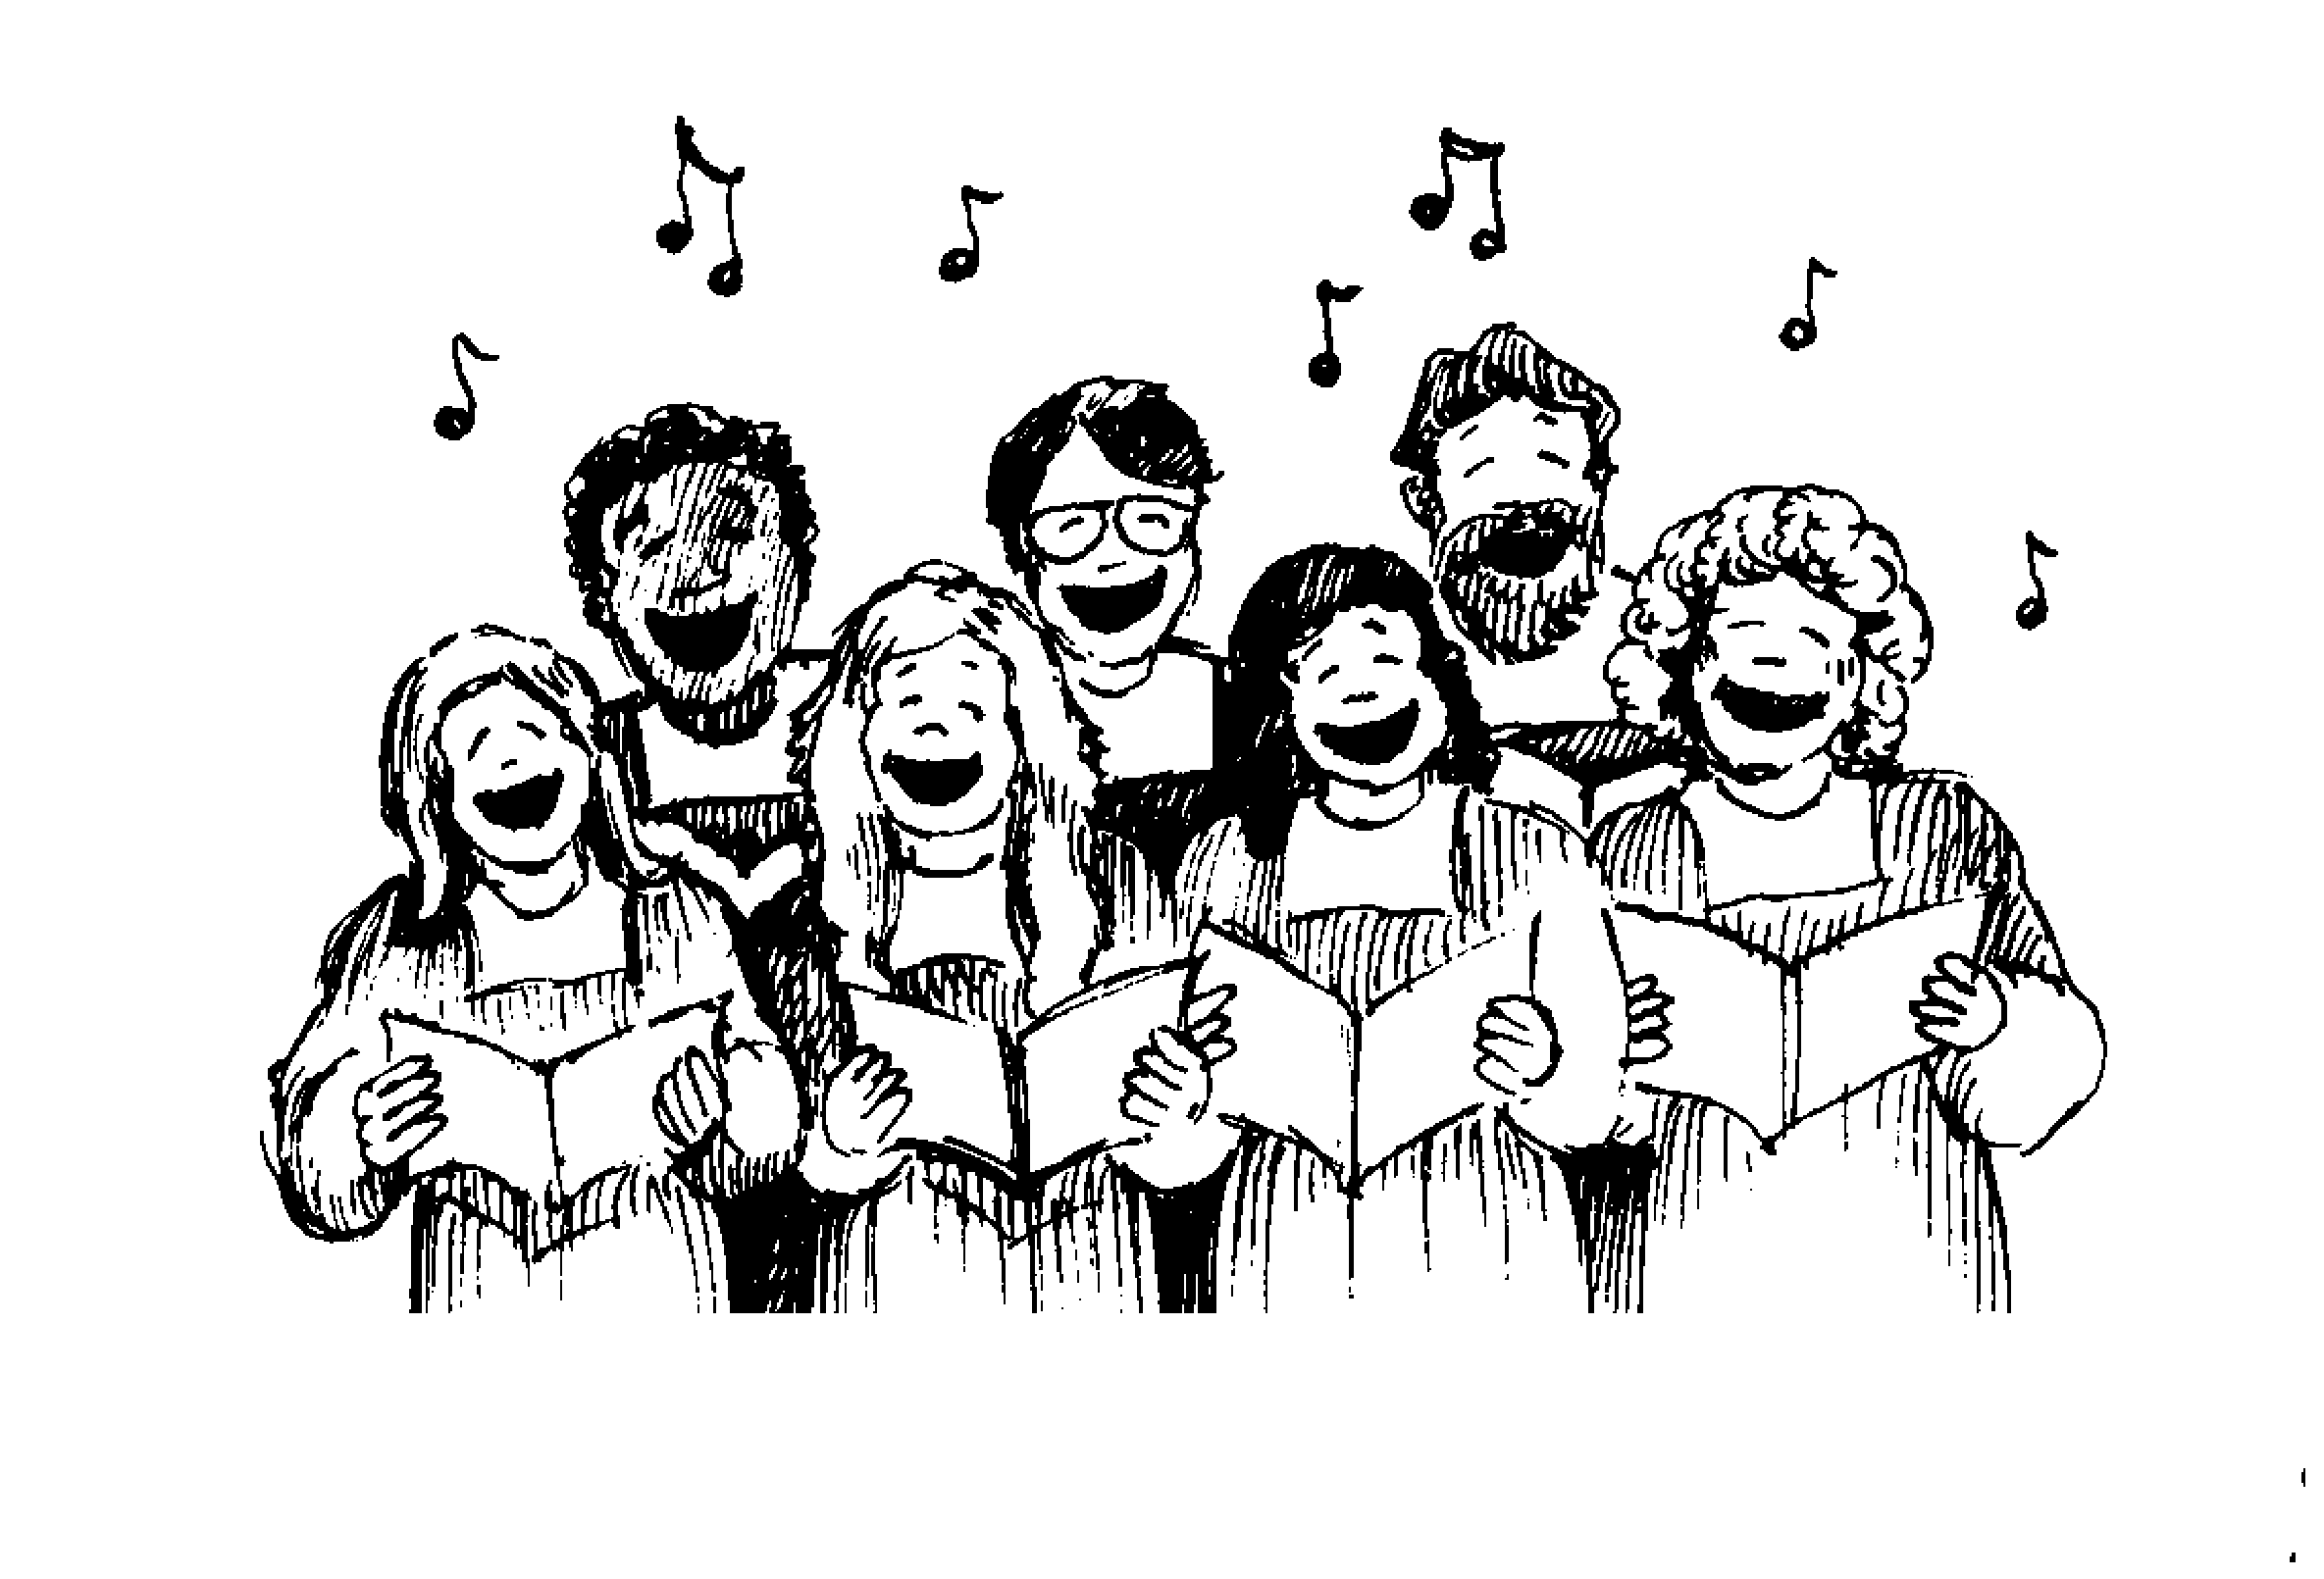
\includegraphics[scale=0.2]{choir01}
\end{center}



\end{document}
